\section{Qualità di prodotto}
Con \strong{qualità} si intende l'insieme delle caratteristiche di un'entità, sia essa un prodotto, un processo o un'intera organizzazione, che ne determinano la capacità di soffisfare esigenze espresse e implicite. Le attività di gestione della qualità costituiscono il \strong{sistema qualità}, con cui si identifica la struttura organizzativa, le responsabilità, le procedure, i procedimenti e le risorse messe in atto per il perseguimento della qualità. Tali attività  si occupano di stabilire un \frgnword{framework} di processi e standard che assicurino un alto livello di qualità, e applicare specifici processi di qualità atti a verificare la corretta aderenza al \frgnword{framework} scelto e la conformità del prodotto finale agli standard.

La qualità di un prodotto è direttamente collegato alla qualità del processo impiegato per crearlo. Approcci come il ciclo di Deming offrono tecniche per specificare obbiettivi di qualità e determinare se essi siano raggiunti.

Vi sono diverse visioni, o punti di vista, da cui valutare la qualità, e su cui il sistema qualità agisce:
\begin{itemize}
	\item Intrinseca: conformità ai requisiti, idoneità all'uso;
	\item Relativa: soddisfazione del cliente;
	\item Quantitativa: misura del livello di qualità per confronto;
\end{itemize}

La qualità software non riguarda quindi solamente il livello di aderenza ai requisiti (aspetti funzionali). La qualità soggettiva di un sistema software dipende principalmente dai suoi attributi non funzionali, come l'affidabilità o l'usabilità, e che riflettono l'esperienza pratica dell'utente. I modelli di qualità, come Bohem o ISO/IEC 9126, definiscono e categorizzano i diversi attributi software. Il piano di qualità deve definire gli attributi ritenuti più importanti per quel prodotto.

\subsection{Gestione della qualità}
Con \strong{gestione della qualità} si intendono le attività del sistema qualità pianificate e attuate affinchè prodotti, servizi e processi soddisfino i requisiti di qualità. Comprende le attività di pianificazione della qualità, \frgnword{quality assurance}, controllo della qualità e miglioramento di processo.

\begin{itemize}
	\item \strong{Pianificazione di qualità}: attività che includono la definizione degli obbiettivi di qualità e degli standard da applicare, la stima dei costi e la pianificazione delle attività di qualità sul calendario.
	\item \strong{\frgnword{Quality assurance}}: attività che definiscono processi e standard che dovrebbero portare a prodotti di alta qualità, introducono processi di qualità nel processo di sviluppo (controllo preventivo della qualità), e accertano l'adeguatezza dei processi software nel fornire il livello di qualità richiesto.
	\item \strong{Controllo della qualità}: attività che esaminano specifici prodotti di progetto per determinare la loro conformità verso gli standard di qualità scelti. Il controllo di qualità esamina sia prodotti intermedi che finali.
	\item \strong{Miglioramento dei processi}: attività che cercano di migliorare l'efficacia e l'efficienza dei processi, con l'obbiettivo ultimo di migliorare la qualità del prodotto software.
\end{itemize}

\paragraph{Pianificazione di qualità}
Le attività di pianificazione di qualità sono mirate a fissare gli obbiettivi e gli standard di qualità, e i processi e le risorse necessarie per conseguirli costituiscono la \strong{pianificazione di qualità}. La pianificazione è prerequisito per ogni altra attività di gestione della qualità, e fissa strategie e politiche sia a livello aziendale che di singolo progetto. E' parte integrante dei processi di sviluppo \frgnword{plan-driven}, mentre viene affrontata in modo meno formale nei modelli agili.

Il processo di pianificazione della qualità sviluppa un piano di qualità per il progetto, che espone le caratteristiche di qualità del software desiderate, e descrive come esse debbano essere valutate.

\subsection{Riferimenti normativi}
Gli standard di qualità del software forniscono strumenti, modelli e metriche per la \strong{definizione} e la \strong{valutazione} della qualità del software, eliminando valutazioni e percezioni soggettive e convertendo priorità astratte e poco chiare in valori quantificabili e misurabili.

\begin{itemize}
	\item Definizione (\strong{modello di qualità}): catalogazione sistematica delle caratteristiche rilevanti;
	\item Valutazione (\strong{metriche}): definizione di metriche per la valutazione delle caratteristiche;
\end{itemize}

Un esempio di standard di qualità è l'ISO/IEC 9126.

\subsubsection{Definizione della qualità: modelli di qualità software}
I modelli di qualità classificano la qualità software in un insieme strutturato di caratteristiche (suddivise ulteriormente in attributi), e costituiscono un modello unico e comune per committenti e fornitori, uniformando la percezione e la valutazione della qualità. Costituiscono strumenti utili alla gestione della qualità mediante valutazione della qualità dei prodotti secondo più punti di vista:

\begin{itemize}
	\item Visione dell'utente, rispetto all'utilizzo pratico;
	\item Visione della produzione, rispetto a qualifica, manutenzione, portabilità e riuso;
	\item Visione della direzione, rispetto al rapporto costi/benefici;
\end{itemize}

Esempi di modelli di qualità sono il modello di Bohem e l'ISO/IEC 9126:2001.

\begin{figure}[h]
	\centering
	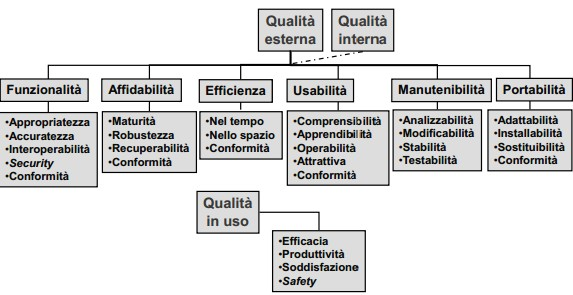
\includegraphics[scale=0.6]{imgs/isoiec_9126_2001.jpg}
	\caption{Caratteristiche di qualità software secondo il modello ISO/IEC9126:2001}
\end{figure}

%\subsubsection{Metriche}

\subsubsection{Standard di qualità}
Gli standard giocano un ruolo molto importante nella gestione della qualità del software. Essi:
\begin{itemize}
	\item Catturano e rappresentano le conoscenze, l'esperienza e le \frgnword{best-practice} dell'azienda;
	\item Forniscono un \frgnword{framework} per l'attuazione di \frgnword{quality assurance};
	\item Supportano la continuità nel momento in cui il lavoro svolto da una persona viene continuato da un'altra: processi standardizzati sono facilmente comprensibili da nuovi assunti;
\end{itemize}

Un uso errato degli standard può avere effetti negativi. E' importante che le norme siano snelle, chiaramente complensibili e supportabili da strumenti automatizzati.
\begin{itemize}
	\item Se gli standard sono poco comprensibili, il personale può percepirli come irrilevanti o bloccanti;
	\item La loro attuazione cieca può comportare eccessi di burocrazia;
	\item Senza il supporto di strumenti informatici, possono richiedere tediose attività manuali;
\end{itemize}

